%%%%%%%%%%%%%%%%%%%%%%%%%%%%%%%%%%%%%%%%%%%%%%%%%%%%%%%%%%%%%%%%%%%%%%%%%%%%%%
%%Skeleton LaTeX file: double column format.
%%%%%%%%%%%%%%%%%%%%%%%%%%%%%%%%%%%%%%%%%%%%%%%%%%%%%%%%%%%%
%%REMEMBER THAT THERE IS AN EIGHT PAGE SIZE RESTRICTION
%%%%%%%%%%%%%%%%%%%%%%%%%%%%%%%%%%%%%%%%%%%%%%%%%%%%%%%%%%%%

%%% Sample file for ME Project Papers for Evaluation by Supervisor and Reader

\documentclass[]{article}


\pagestyle{empty}
\setlength{\topmargin}{ 0.25in}
\setlength{\columnsep}{2.0pc}
\setlength{\headheight}{0.0in}
\setlength{\headsep}{0.0in}
\setlength{\oddsidemargin}{-.19in}
\setlength{\parindent}{1pc}
\textheight 8.75in
\textwidth 6.8in

\usepackage{multicol}
\usepackage{graphics}
\usepackage[numbers]{natbib}
\usepackage{url}

\usepackage{color,float}
\usepackage{boxedminipage}
\usepackage{epsfig} 
\usepackage{amsmath}
\usepackage{amssymb}
\usepackage{amsfonts}
\usepackage{comment}
\usepackage{tikz}
\usetikzlibrary{patterns}
\usepackage{subfig}
\DeclareCaptionType{copyrightbox}
\usepackage{algorithm}
\usepackage{algorithmic}
\usepackage{eqparbox}
\usepackage{times}

\newenvironment{Figure}
  {\par\medskip\noindent\minipage{\linewidth}}
  {\endminipage\par\medskip}

\title{\large \bf On Demand Data Generation at Big Data Scale}
\author{Raghav Sood \\ Computer Science and Automation \\ Indian Institute of Science Bangalore \\ raghav@dsl.serc.iisc.ernet.in}

\date{July 18, 2016}

\begin{document}

    \maketitle
    \begin{center}
        Mid-term ME Project Report
    \end{center}
        \vskip 12pt
	\thispagestyle{empty}
	
	\begin{abstract}
		OLAP engines are used widely in large data warehousing environments for Business Intelligence and Data Mining. 
		To evaluate and test these engines, we need to have synthetic data with specific characteristics. 
		TPC-DS \cite{tpcds} is an industry standard benchmark for Big Data systems but it represents only a particular data scenario. This limits its ability to capture various realistic customer scenarios. 
		Other challenge in large scale synthetic data generation is the space and time overhead involved in storing and indexing generated data. This makes the traditional techniques of data generation simply impractical at Big Data scale. 
		We have developed an approach to \textit{generate synthetic data} having \textit{custom characteristics}. Also the generation is \textit{on demand} thereby mitigating the space and time overheads. 

		Our approach takes database schema and data characteristics expressed as set of \textit{cardinality constraints} \cite{arasu} as input. 
		These constraints can be user specified or can also be inferred from output cardinality of all intermediate operators appearing in a given set of Query Plans. 
		Given these cardinality constraints, our approach can then synthetically generate a \textit{virtual} database instance, which for workload queries, behaves "exactly" like the client's database. The behaviour here is in volumetric terms i.e., getting the same number of output tuples at each intermediate operator in the query plan. 
		This ability to mimick a client's data scenario at the development site will be very useful in database engine testing in particular and data masking in general.
		The approach also gives the ability to mimick scaledup versions of the client's database making it highly helpful in analyzing futuristic scenarios. 
		 
	\end{abstract}	
	
	\hfill \\
	
	\begin{multicols}{2}
	\section{Introduction}
		A database engine has broadly two components- the \textit{query optimizer} aka. planner and the \textit{executor}.
		A query is processed in two phases. 
		Compile-time processing is where given a query the optimizer comes up with an optimal plan. 
		Thereafter, at execution-time, the executor runs the given plan and produces result.
		Therefore, testing of database engine can be categorized into \textit{compile-time testing} and \textit{execution-time testing}.
		And effective testing is predicated on the ability to easily construct alternative scenarios with regard to the database contents \cite{codd}. 
		Our work is concerned with data generation which can be used for performance testing of the executor.  
		
		The already available synthetic benchmarks like TPC-H \cite{tpch}, TPC-DS \cite{tpcds} are commonly used to carry out performance tests in various domains. 
		But a benchmark like these represents only a particular data scenario. 
		The corresponding generators provided by TPC offer an option to generate various scaled versions of the benchmarks, say- 1, 3, 10, 30 or 100 TB for TPC-DS.
		Whereas extremely limited or no option is offered to change the distribution of the data or manipulate correlation accross columns or relations. 
		This is because of the fundamental reason that allowing such an option defeats the benchmark's purpose of objective and verifiable evaluation of systems. 
		Unfortunately, it makes these benchmarks far from various realistic customer scenarios to which a database vendor serves. 
		However, often these benchmarks are the only possibility, as customer data and workloads are hard to obtain, due to their sensitive nature and moreover they are usually very large which makes transmission over the network hard if not impossible \cite{rsgen}.
		This may endup with unidentified bugs getting deployed. 

		Recent work \cite{arasu} has proposed generating \textit{workload-aware} datasets with the help of constraint solvers. 
		However, this does not scale well to the amounts of data typically present in a customer dataset \cite{rsgen}. 
		Another recent work RSGen \cite{rsgen} is on generating data by \textit{reversing metadata statistics}. 
		This techniques works well in terms of recovering the metadata statistics and in terms of volumetric similarity of COUNT queries on single columns.
		However, data generated by this technique shows discrepencies for queries which go beyond the simple independent range queries. 
		Thus data generated by RSGen works for analyzing the behavior of query optimizer since it has fundamentally the same metadata characteristics. 
		But this data cannot be used to analyze the performance of executor because execution of a query depends highly on the \textit{fine-grained data characteristics} which are the operator level volumetric outputs at each intermediate stage of a query plan. 
		Refer section 6 for a detailed discussion on related work. 
		
		We present a scalable approach to synthetically generate a database instance which has given fine-grained data characteristics. 
		As an input to our approach, the desired data characteristics are specified in a natural, expressive and declarative manner called \textit{cardinality constraints} \cite{arasu}. 
                These constraints can be user specified or can also be inferred from a given set of Query Plans. 
                The workload for any database client application usually consists of a fixed set of queries. 
                And on an existing client database, running the \textit{explain analyze} command (in case of PostgreSQL or its equivalent in case of other engines) for workload queries gives the output cardinality of all intermediate operators as witnessed during the course of execution of the query. 
                Starting PostgreSQL version 9.0, this command outputs in program readable formats (xml/json/yml) which makes it very easy to capture the fine-grained data characteristics as cardinality constraints. 
		Our approach solves these cardinality constraints along with the referential integrity constraints imposed from the schema. 
		The solution to these constraints is represented as \textit{database summary} which is in order of megabytes while the original database could be in terabytes to petabytes.
		This database summary is next used as a seed to our on-demand synthetic tuple generator. 
		
		We are hence able to synthetically generate a \textit{virtual} database instance, which for workload queries, behaves "exactly" like the client's database. 
		The behaviour here is in volumetric terms i.e., getting the same number of output tuples at each intermediate operator in the query plan. 
                
		This ability to mimick a client's data scenario at the database vendor's development site will be very useful for database engine testing.
		Also the approach serves as a Data Masking technique. Organisations which outsource the testing of their database applications may now share the database summary. 
		The approach also gives the ability to mimick scaledup versions of the client's database making it highly helpful in analyzing performance in futuristic scenarios. 
	
	\section{Preliminaries}
	        \subsection{Annotated Query Plan (AQP)}
		A logical query plan is an extended relational algebra tree. It gives the set of operations involved in executing a query as per their sequence. For example, consider the following sql query on TPC-DS schema: 
		\\ \\
			\fbox{\parbox[c][7em][c]{\linewidth}{
				select * from \\ 
				web\_sales W, date\_dim D, item I \\ 
				where D.d\_month\_seq $>$= 1211 \\ 
				and W.ws\_sold\_date\_sk = D.d\_date\_sk \\ 
				and W.ws\_item\_sk = I.i\_item\_sk
			}}
		\\ \\
		An AQP is a logical query plan which in addition also gives input and output cardinalities for each operator in the tree. 
		The input cardinality specifies the number of tuples that reach the operator and the output cardinality gives the number of tuples that leave the operator. 

			\begin{Figure}
				\centering
				
\includegraphics[width=2in]{figures/alqp1.png}
				\captionof{figure}{Annotated Query Plan (AQP)}
				\label{fig:mso_bound}
			\end{Figure}


		
		\subsection{Cardinality Constraints}
		Assuming that $\mathcal{R}_1, ... , \mathcal{R}_l$ are the set of relations in the database, each operator in the AQP corresponds to a cardinality constraint that can be written in the following form:
			\[ | \pi_\mathcal{A} \sigma_\mathcal{P} (\mathcal{R}_{i_1} \bowtie ... \bowtie \mathcal{R}_{i_p}) | = k\]
		where $\mathcal{A}$ denotes a set of attributes, $\mathcal{P}$ is a selection predicate, and $k$ is a non-negative integer.
		For example, the constraints corresponding to the AQP shown in Figure 2.2 are:
			\begin{equation*}
				|W| = 7197559
			\end{equation*}
			\begin{equation*}
				|D| = 73066
			\end{equation*}
			\begin{equation*}
				|I| = 102006
			\end{equation*}
			\begin{equation*}
				|\sigma_{d\_month\_seq >= 1211}(D)| = 36192
			\end{equation*}
			\begin{equation*}
				|\sigma_{d\_month\_seq >= 1211}(W \bowtie D)| = 3131870
			\end{equation*}
			\begin{equation*}
				|\sigma_{d\_month\_seq >= 1211}(W \bowtie D \bowtie I)| = 3131870
			\end{equation*}

	\section{Problem}
		\subsection{Statement}
		We shall now formally state the problem:
		\\ \\
			\fbox{\parbox[c][5em][c]{\linewidth}{
				Given a database schema $\mathcal{S}$ and a set of AQPs  $\mathcal{W}$, generate a database instance that conforms to $\mathcal{S}$ and satisfies all the cardinality constraints ($\mathcal{C}_1, \mathcal{C}_2, ... , \mathcal{C}_m$) generated from $\mathcal{W}$.
			}}
		\\ \\
		In the decision version \footnote{In the decision version of the problem, the output is YES if there exists a database instance that satisfies all the constraints and NO, otherwise} of this problem is \textit{NEXP-complete} \cite{arasu}.
		
		\subsection{Assumptions}
		The assumptions made in our work are:
			\begin{itemize}
				\item All the joins appearing in the constraints are {\em primary key-foreign key} joins.
				\item The dependency (due to joins) between relations should be {\em non-cyclic}.
				\item Selection predicates include only non-key attributes.
			\end{itemize}

	\section{Data Generation}
		Our data generator takes the schema of the desired database as the input. 
		Along with it, the set of ALQPs are also given as the input. 
		The AQPs are generated after executing the queries on the original database. 
		These AQPs can be easily fetched from the execution-plan information that the database engines provide. 
		The generator uses these inputs to give the synthetic database (on-the-fly) as the output. 
		We next describe the architecture of the generator.

		\subsection{Architecture}
		Figure 3.1 provides an overview of the architecture of the data generator. 
		Its various components are:
		
		\begin{Figure}
			\centering
			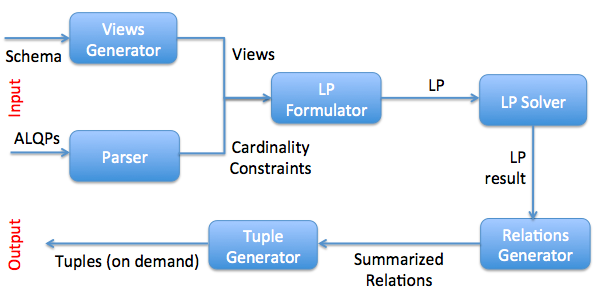
\includegraphics[width=2in]{figures/architecture.png}
			\captionof{figure}{Architecture}
			\label{fig:Architecture}
		\end{Figure}
		
		\begin{itemize}
			\item {\bf Parser:} 
			The purpose of parser is to take $\mathcal{W}$ as input and give the set of cardinality constraints as described in Section 2.1.3. 
			Note that for now we are not considering projection operator. 
			Therefore, all the constraints will be of the form:
			\begin{equation*}
			| \sigma_\mathcal{P} (\mathcal{R}_{i_1} \bowtie ... \bowtie \mathcal{R}_{i_p}) | = k
			\end{equation*}
		
			\item {\bf View Generator:} 
			This component takes the database schema as input and creates a view $\mathcal{V}_{i}$ corresponding to every relation $\mathcal{R}_{i}$. 
			Creation of views help us to get rid of the join expressions in the constraints, i.e., once the views are created, each constraint can be re-written as a selection predicate over a single view only. 
			We shall see this component in detail in Section 3.2.1.
		
			\item {\bf LP Formulator:} 
			This component uses the views given by the view generator to re-write the cardinality constraints given by the parser. 
			Further, an LP is created for each view. This is done by converting each constraint (on that view) to a corresponding equation. 
			Once this is done, the system of equations is passed on to the LP solver. 
			We shall discuss the details of constructing equations in detail in Section 3.2.2.
		
			\item {\bf LP Solver:} 
			This component takes the system of equations and gives one of the feasible solutions
			\footnote{The system of equations can have infinite solutions. 
			The solution corresponding to the original database instance might differ from the solution we get here. But, both the solutions would satisfy all the constraints.}. 
			We use the GNU Linear Programming Kit (GLPK) \cite{glpk} for solving the LP. 
		
			\item {\bf Relation Generator:} 
			This component takes the solution given by the LP solver and 
				(i) makes it consistent across the views, 
				(ii) constructs compressed relations from it, which is sufficient to generate the entire relation. 
			Section 3.2.3 discusses this component in detail.
		
			\item {\bf Tuple Generator:} 
			The compressed relations that we obtain from the relations generator serve as the seeds to the tuple generator. 
			The tuple generator has the capability of generating a tuple(s) on demand for any relation $\mathcal{R}_{i}$. 
			The detailed description of this component is mentioned in Section 3.2.4.
		
		\end{itemize}
	
		\subsection{Details}
			\subsubsection{View Generator}
			As discussed earlier, the purpose of this component is to simplify the constraints such that we can replace all the join expressions by a single view. 
			For this we need to construct a view $\mathcal{V}_{i}$ corresponding to each relation $\mathcal{R}_{i}$. 
			A view $\mathcal{V}_{i}$ can be considered as a set of non-key attributes that are present in either $\mathcal{R}_{i}$ or in any other relation on which $\mathcal{R}_{i}$ depends. 
			The dependencies between relation can be seen from the {\em dependency graph}.
			
			{\bf Dependency Graph:} 
			In a dependency graph, we create a node for every relation. 
			A directed edge from a node $\mathcal{R}_{i}$ to $\mathcal{R}_{j}$ is added, if $\mathcal{R}_{i}$ contains a {\em foreign-key} referencing $\mathcal{R}_{j}$.
			
			Now, a relation $\mathcal{R}_{i}$ is said to be dependent on relation $\mathcal{R}_{j}$ if there exists a path from $\mathcal{R}_{i}$ to $\mathcal{R}_{j}$ in the dependency graph.
		
			Let us see the following example: Consider a database having following four relations:
			\\ \\
			\fbox{\parbox[c][8em][c]{\linewidth}{
				\begin{equation*}
				Catalog\_sales (\underline {PK_{1}}, FK_{C}, FK_{D}, cs\_sales\_price)
				\end{equation*}
				\begin{equation*}
				Date\_dim (\underline {PK_{3}}, d\_qoy, d\_year)
				\end{equation*}
				\begin{equation*}
				Customer (\underline {PK_{2}}, FK_{CA})
				\end{equation*}
				\begin{equation*}
				Customer\_address (\underline {PK_{4}}, ca\_state
				\end{equation*}
			}}
			\\ \\
			Here, $PK_{1}$, $PK_{2}$, $PK_{3}$, $PK_{4}$ are the primary keys of the respective relations. 
			$FK_{C}$ references to $Customer$, $FK_{D}$ references to $Date\_dim$ and $FK_{CA}$ references to $Customer\_address$. 
			Therefore, the dependency graph would be as shown in Figure 3.2. 
			
			\begin{Figure}
				\centering
				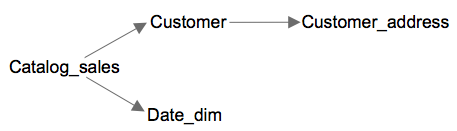
\includegraphics[width=2in]{figures/schema_dig.png}
				\captionof{figure}{Dependency Graph}
				\label{fig:dependency-graph}
			\end{Figure}
	
			By traversing the dependency graph in reverse topological sort order and a view corresponding to each relation is generated. 
			\\ \\
			\fbox{\parbox[c][8em][c]{\linewidth}{
				\begin{equation*}
				Catalog\_sales' (ca\_state, d\_qoy, d\_year, cs\_sales\_price)
				\end{equation*}
				\begin{equation*}
				Date\_dim' (d\_qoy, d\_year)
				\end{equation*}
				\begin{equation*}
				Customer' (ca\_state)
				\end{equation*}
				\begin{equation*}
				Customer\_address' (ca\_state)
				\end{equation*}
			}}
			\\ \\
	
			\subsubsection{LP Formulator}
			The LP Formulator receives the set of constraints from the parser and the set of views from the view generator. 
			The first task it does is to re-write the constraints by replacing the join expressions with appropriate views. 
			Say we have a constraint having join: $\mathcal{R}_{i} \bowtie \mathcal{R}_{k}$. 
			Since, we have assumed that all joins are of primary key-foreign key type, one of these is a dependent relation. 
			Say $\mathcal{R}_{i}$ depends on $\mathcal{R}_{k}$. 
			In such a case, we shall replace the expression $\mathcal{R}_{i} \bowtie \mathcal{R}_{k}$ with $\mathcal{V}_{i}$. 
			Because of the way we constructed the views, it is easy to see that we can apply the predicate that was there on  $\mathcal{R}_{i} \bowtie \mathcal{R}_{k}$ to $\mathcal{V}_{i}$. 
			Likewise, all the join expressions can be expressed in terms of a single view respectively.
			
			Continuing on the example as in Figure 2.2, considering that the dependency graph is rooted at node $W$ having two children $D$ and $I$, the cardinality constraints 2.5 and 2.6 can be rewritten as:
			\begin{equation*}
				|\sigma_{d\_month\_seq >= 1211}(W')| = 3131870
			\end{equation*}
			\begin{equation*}
				|\sigma_{d\_month\_seq >= 1211}(W')| = 3131870
			\end{equation*}
			where $W'$ represents the view corresponding to $W$.
			
			
			So now we can solve for each view separately. 
			For each view $\mathcal{V}_{i}$, we will find the set of constraints imposed on $\mathcal{V}_{i}$. 
			A constraint $\mathcal{C}_{j}$ on $\mathcal{V}_{i}$ will be of the following form:
			\begin{equation*}
				| \sigma_{\mathcal{P}_{j}} (\mathcal{V}_{i})| = k_{j}
			\end{equation*}
			
			Now, let us assume we have a single view $\mathcal{V}$ having a set of attributes $A_{1}$, $A_{2}$,...,$A_{n}$. 
			We need to formulate an LP for the view $\mathcal{V}$. 
			Let the domain of an attribute $A_{i}$ be represented by $Dom(A_{i})$. 
			We assume that the domain of all the attributes are positive integers bounded by an integer $D$. 
			For attributes with non-integral domains, we can map the values to integers. 
			This assumption is to simplify the analysis and can be removed easily.
			
			Say we are given a set of $m$ constraints that $\mathcal{V}$ satisfies. 
			Each constraint $C_{j}$  $(1 \leq j \leq m)$ for simplicity can be expressed as: $<\mathcal{P}_{j}, k_{j}>$, which means that the number of tuples (rows) satisfying the condition $\mathcal{P}_{j}$ is equal to $k_{j}$. 
			
			For every tuple $t \in Dom(A_{1}) \times Dom(A_{2})\times...\times Dom(A_{n})$, we create a variable $x_{t}$ representing the number of copies of $t$ in $\mathcal{V}$. 
			Now, for each of the $m$ constraints $C_{j}$ $(1 \leq j \leq m)$, we create a linear equation:
			\begin{equation*}
				\sum_{t:P_{j}(t)=true} x_{t} = k_{j}
			\end{equation*}
			
			In addition, we also require that $x_{t} \geq 0$ $\forall t$ as the number of tuples are always non-negative integers. 
			Since, the solution of the LP need not be integral, we shall use simple {\em rounding technique}. 
			
			Further, since the number of variables in the LP is proportional to the domain size, which can be huge, there are some optimizations that can be done to reduce the size of the LP. 
			We will now discuss these optimizations.
	
	
			\subsubsection{Domain Decomposition}
			A set $v^{i}$ is created for each attribute $A_{i}$. 
			Values in  $v^{i}$ are added according to the following: 
			We iterate over the constraints and if a constraint has
			
			\begin{itemize}
				\item $A_{i} >= a$ or $A_{i} < a$, we add $a$ in  $v^{i}$.
				\item $A_{i} > a$ or  $A_{i} <= a$, we add $a + 1$ in $v^{i}$.
				\item $A_{i} = a$, we add $a$ and $a+1$ both in $v^{i}$.
			\end{itemize}
			
			All the other constraints can be expressed as combinations of the above. 
			In addition, we also add $1$ (minimum value in domain) in $v^{i}$ if not already present. 
			Let  $v_{1}^{i}, v_{2}^{i},...,v_{l_{i}}^{i}$ represent the constants (in increasing order) in the set $v^{i}$. 
			Now we can divide the domain of an attribute $A_{i}$ into a set of $l_{i}$ intervals $I^{i}: [v_{q}^{i},v_{q+1}^{i})$ $(1 \leq q < l_{i}) \cup [v_{l_{i}}^{i},)$. 
			The semantics of the variables can now be modified such that we introduce a variable $x_{t'}$ for each interval combination $t' \in I^{1} \times I^{2} \times ... \times I^{n}$, representing the number of tuples lying in the interval combination $t'$.
			
			Therefore, now for each constraint $C_{j}$ $(1 \leq j \leq m)$, the linear equation would be:
			\begin{equation*}
				\sum_{t':P_{j}(t')=true} x_{t'} = k_{j}
			\end{equation*}
			Here as well we will have the additional constraint of $x_{t'} > 0$ $\forall t'$.
			
			{\em Example:} 
			Let us see the LP formulation for relation $Catalog\_sales$ having following constraints:
			\begin{equation*}
				|CS| = 14401261
			\end{equation*}
			\begin{equation*}
				|\sigma_{cs\_sales\_price > 150} (CS)| = 734606
			\end{equation*}
			\begin{equation*}
				|\sigma_{cs\_sales\_price > 150 \wedge ca\_state = 1} (CS)| = 13806
			\end{equation*}
			These constraints can be converted into the corresponding LP equations as follows:
			\begin{equation*}
				x_{[1,151)[1,2)} + x_{[1,151)[2,)} + x_{[151,)[1,2)} + x_{[151,)[2,)} = 14401261
			\end{equation*}
			\begin{equation*}
				x_{[151,)[1,2)} + x_{[151,)[2,)} = 734606
			\end{equation*}
			\begin{equation*}
				x_{[151,)[1,2)} = 13806
			\end{equation*}
			
			Therefore, we can see that by applying this optimization, the number of variables are a function of the size of the sets $v^{i}s$ instead of the domain size. 
			But, even after applying this optimization, the number of variables are exponential in the number of attributes. 
			To further reduce the LP's complexity, we will next look at another optimization that tries to decompose the view into smaller views.
			
			
			\subsection{Relation Generator}
			The LP solver gives the result for each clique $c_{i}$ in the form of the set:
			\[\{(x, k_{x}^{i})\}_{x \in Dom(\mathcal{A}_{c_{i}})}\]
			where $x$ represents an interval combination and $k_{x}^{i}$ represents the number of tuples in the view that lie in the interval combination $x$. 
			Note that $x$ constitutes of intervals of those attributes that are present in $\mathcal{A}_{c_{i}}$.
			
			Since, the above solution has intervals for a set of attributes, to get a value combination from this, we need to pick a value from each interval. 
			We pick the minimum value in every interval to get the value combination. 
			We do this to minimize the error that is incurred in the view consistency algorithm (we shall discuss this in Section 3.2.3.2)
			\footnote{any deterministic method of picking a value in an interval can be adopted to reduce the error}. 
			Now on we shall use $x$ to represent the value combination thus obtained.
			
			Let us call these solution sets as the {\em clique-solution sets}. 
			We might not explicitly mention it always, but when we say $x \in Dom(\mathcal{A}_{c_{i}})$, we consider only those domain values for which the corresponding $k_{x}^{i}$ is non-zero since we do not need to store the domain values that do not occur from our LP solution.
			
			The relation generator does the following:
			\begin{itemize}
				\item First, it merges the clique-solution sets to obtain the solution for the complete view.
				\item Then, it makes the views consistent.
				\item Finally, it constructs relation summaries.
			\end{itemize}
			
			
			\subsubsection{Obtaining View Solution}
			The solution for the complete view is obtained by {\em merging the cliques} (Algorithm 2). 
			This is done by first ordering the cliques using the {\em Order Cliques Procedure} (Algorithm 3). 
			This merge ordering is necessary in order to retain all the constraints that each clique solution implies. 
			In every iteration of ordering algorithm, we look for a clique $c_{i}$ that is independent of the observed cliques so far except for the attributes that are common between $c_{i}$ and the observed cliques. 
			Since the graph is chordal, we are guaranteed to get at least one such ordering. 
			
			Once we get the ordering, we then merge the cliques-solution sets one by one in that order. 
			Merging is a three step process. 
			We first sort the clique-solution sets based on their common attributes, then use the {\em Align Procedure} (Algorithm 4) to split the rows in the two clique-solution sets in such a way that the corresponding rows in the two sets have same values for the number of tuples entry. 
			Finally we join the two sets using the {\em Merge Procedure} (Algorithm 5).
			
			{\em Example:} Consider a case where we need to merge two clique-solution sets to obtain a view solution set. Let the two clique-solution sets be as follows: \\
			\end{multicols}
			
			\begin{tabular}{ p{0.5\textwidth} p{0.5\textwidth} }
				
				\begin{tabular}{ |p{1.6cm}|p{1.6cm}|p{1.6cm}|}
					\hline
					\multicolumn{3}{|c|}{Clique-solution 1} \\
					\hline
					A & B & number of tuples \\
					\hline
					10 & 20 & 100 \\
					30 & 50 & 60 \\
					10 & 50 & 40 \\
					30 & 20 & 200 \\
					\hline
				\end{tabular}

				&

				\begin{tabular}{ |p{1.6cm}|p{1.6cm}|p{1.6cm}|}
					\hline
					\multicolumn{3}{|c|}{Clique-solution 2} \\
					\hline
					B & C & number of tuples \\
					\hline
					20 & 5 & 150 \\
					50 & 15 & 100 \\
					20 & 15 & 150 \\
					\hline
				\end{tabular}
			
				\\
	
				\multicolumn{2}{l}{After sorting on common attribute attribute B, we would obtain:} 
			
				\\
			
				\begin{tabular}{ |p{1.6cm}|p{1.6cm}|p{1.6cm}|}
					\hline
					\multicolumn{3}{|c|}{Clique-solution 1} \\
					\hline
					A & B & number of tuples \\
					\hline
					10 & 20 & 100 \\
					30 & 20 & 200 \\
					10 & 50 & 40 \\
					30 & 50 & 60 \\
					\hline
				\end{tabular}
			
				&
			
				\begin{tabular}{ |p{1.6cm}|p{1.6cm}|p{1.6cm}|}
					\hline
					\multicolumn{3}{|c|}{Clique-solution 2} \\
					\hline
					B & C & number of tuples \\
					\hline
					20 & 5 & 150 \\
					20 & 15 & 150 \\
					50 & 15 & 100  \\
				 	\hline
				\end{tabular}
			
				\\
			
				\multicolumn{2}{l}{After aligning the two sets, we obtain:} 
			
				\\
			
				\begin{tabular}{ |p{1.6cm}|p{1.6cm}|p{1.6cm}|}
					\hline
					\multicolumn{3}{|c|}{Clique-solution 1} \\
					\hline
					A & B & number of tuples \\
					\hline
					10 & 20 & 100 \\
					30 & 20 & 50 \\
					30 & 20 & 150 \\
					10 & 50 & 40 \\
					30 & 50 & 60 \\
					\hline
				\end{tabular}
			
				&
			
				\begin{tabular}{ |p{1.6cm}|p{1.6cm}|p{1.6cm}|}
					\hline
					\multicolumn{3}{|c|}{Clique-solution 2} \\
					\hline
					B & C & number of tuples \\
					\hline
					20 & 5 & 100 \\
					20 & 5 & 50 \\
					20 & 15 & 150 \\
					50 & 15 & 40 \\
					50 & 15 & 60\\
					\hline
				\end{tabular}
			
				\\
			
				\multicolumn{2}{l}{Finally, after merging, the view solution set thus obtained is:} 
			
				\\
			
				\begin{tabular}{ |p{1.6cm}|p{1.6cm}|p{1.6cm}|p{1.6cm}|}
					\hline
					\multicolumn{4}{|c|}{View solution} \\
					\hline
					A & B & C & number of tuples \\
					\hline
					10 & 20 & 5 & 100 \\
					30 & 20 & 5 & 50 \\
					30 & 20 & 15 & 150 \\
					10 & 50 & 15 & 40 \\
					30 & 50 & 15 & 60 \\
					\hline
				\end{tabular}
			
				&
			
	 		\end{tabular}
			
	\pagebreak
	\begin{multicols}{2}
	
	\section{2nd SECTION TITLE}
%		\begin{algorithm}
%		\begin{algorithmic}             
%			\STATE \textbf{Init:} i=1, $\epps=\{e_1, \ldots, e_D\}$;
%			\WHILE[\hspace*{0.1in} for each contour]{$i \le m$}
%			\IF[\hspace*{0.1in}  only one ${\epp}$ left]{$|\epps|= 1$}
%			\STATE Run {\pb} to discover the selectivity of the remaining ${\epp}$ starting from the \emph{present} contour;
%			\STATE Exit;
%			\ENDIF
%			\STATE Run the spill node identification procedure on each plan in the contour $\ic{i}$, i.e, plans in $\pl{{i}}$, and use this information to choose plan $\plmax{j}$ for each ${\epp}$ $e_j $;
%			\STATE exec-complete  =  false;  
%			\FOR{\textbf{each} ${\epp}$ $e_j$} 
%			\STATE {\normalsize exec-complete = Spill-Mode-Execution($\plmax{j}$,$e_j$,$\icc{i}$)};
%			\STATE Update ${{\rp.j}}$ based on selectivity learnt for $e_j$; 
%			\IF{exec-complete}
%			    \STATE /*learnt the actual selectivity for $e_j$*/ 
%			    \STATE Remove $e_j$ from the set $\epps$;
%			    \STATE Break; 
%			\ENDIF
%			\ENDFOR
%			\IF{!\;exec-complete}
%			\STATE i = i+1; /* Jump to next contour */ 
%			\ENDIF
%			\STATE Update ${\ess}$ based on learnt selectivities;
%			\ENDWHILE
%		\end{algorithmic}
%		\caption{The {\sbd} Algorithm} ~\label{algo:multidSpillBound}
%		\end{algorithm}
%%%%%%%%%%%%%  This can be followed by several other sections

	\section{Conclusions and Future Work}
	Proin id elit nec erat pellentesque gravida ut a lectus. Proin rhoncus eu justo et aliquet. Praesent auctor augue quis magna dapibus imperdiet. Fusce vehicula vehicula aliquet. Fusce ac dolor in lorem tristique bibendum eget finibus turpis. In odio dui, mattis sed commodo non, bibendum et augue. Nam dignissim id metus ut bibendum. Nulla eu leo sed dui venenatis viverra. Donec et enim rutrum lorem aliquam bibendum ac ac arcu. Lorem ipsum dolor sit amet, consectetur adipiscing elit. In gravida enim vitae nisi tincidunt pulvinar. Maecenas hendrerit lacinia dui, et egestas turpis suscipit sed. Vestibulum eros orci, bibendum in diam in, suscipit aliquet ipsum. Nulla facilisi. Vestibulum vulputate, nulla ut ornare varius, eros leo elementum sem, at tempor ante massa vitae dolor.	


\bibliographystyle{plainnat}
\bibliography{references}
	
\end{multicols}
\end{document}
